\documentclass{beamer}
\usetheme{metropolis}
\usepackage{graphicx}
\usepackage{subfig}
\usepackage{tcolorbox}
\title{Algebra-Based Physics-2: Electricity, Magnetism, and Modern Physics: Unit 3}
\author{Jordan Hanson}
\institute{Whittier College Department of Physics and Astronomy}

\begin{document}
\maketitle

\section{Summary}

\begin{frame}{Unit 2 Summary}
\textbf{Reading: Chapter 22}
\begin{enumerate}
\item Magnets and magnetic fields
\item Force on a moving charge in a magnetic field
\item Magnetic forces on conductors
\item \alert{The Hall effect}
\item \alert{Amp\`{e}re's Law}
\end{enumerate}
\end{frame}

\section{Magnets and magnetic fields}

\begin{frame}{Magnets and magnetic fields}
Introductory video on the origin of magnetic fields and forces they exert on charge: \\ \vspace{0.5cm}
\url{https://www.youtube.com/watch?v=s94suB5uLWw}
\end{frame}

\begin{frame}{Magnets and magnetic fields}
What is a cross-product and how does it work? \\ \vspace{0.25cm}
\begin{figure}
\centering
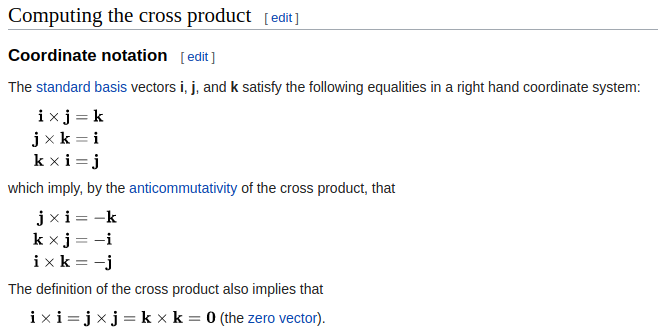
\includegraphics[width=0.75\textwidth]{figures/crossP.png}
\caption{\label{fig:crossP} The cross-product is a way of multiplying unit vectors.}
\end{figure}
\textbf{Professor:} several examples on board.
\end{frame}

\begin{frame}{Magnets and magnetic fields}
Let $\vec{v} = 2\hat{i}$ and $w = -2 \hat{j}$.  What is $\vec{v} \times \vec{w}$?
\begin{itemize}
\item A: $-4 \hat{k}$
\item B: $4 \hat{k}$
\item C: $-2 \hat{i}$
\item D: $2 \hat{j}$
\end{itemize}
\end{frame}

\begin{frame}{Magnets and magnetic fields}
Let $\vec{v} = 3\hat{j}$ and $w = 5 \hat{k}$.  What is $\vec{v} \times \vec{w}$?
\begin{itemize}
\item A: $15 \hat{i}$
\item B: $5 \hat{j}$
\item C: $3 \hat{i}$
\item D: $15 \hat{k}$
\end{itemize}
\end{frame}

\begin{frame}{Magnets and magnetic fields}
Let $\vec{v} = 3\hat{i} \times 3\hat{j}$ and $w = 2 \hat{k}$.  What is $\vec{v} \times \vec{w}$?
\begin{itemize}
\item A: $-6 \hat{j} + 6\hat{k}$
\item B: $-6 \hat{j} + 6\hat{i}$
\item C: $6 \hat{j} + 6\hat{i}$
\item D: $6 \hat{k} + 6\hat{i}$
\end{itemize}
\end{frame}

\begin{frame}{Magnets and magnetic fields}
\textbf{Group exercise:} Compute the following cross product:
\begin{align}
\vec{v} &= 2\hat{i}-2\hat{j} \\
\vec{w} &= 4\hat{j}-4\hat{i} \\
\vec{v} \times \vec{w} &= ??
\end{align}
\end{frame}

\begin{frame}{Magnets and magnetic fields}
\textbf{Group exercise:} Compute the following cross product:
\begin{align}
\vec{v} &= 2\hat{i}-2\hat{j}+\hat{k} \\
\vec{w} &= 4\hat{j}-4\hat{i}-\hat{k} \\
\vec{v} \times \vec{w} &= ??
\end{align}
\end{frame}

\begin{frame}{Magnets and magnetic fields}
\begin{tcolorbox}[colback=white,colframe=black!100!black,title=The Lorentz Force]
\alert{Let a particle with charge $q$ and velocity $\vec{v}$ move through a \textit{magnetic field} $\vec{B}$.  The \textbf{Lorentz force} on the charged particle is
\begin{equation}
\vec{F}_{\rm L} = q\vec{v} \times \vec{B}
\label{eq:Lorentz}
\end{equation}}
\end{tcolorbox}
\textit{As a helpful memory tool, we have the right-hand rule to remember the direction of the cross-product.}  \textbf{The units of the magnetic field are the Telsa}, after Nikola Tesla.  We also have the Gauss which is $10^{-4}$ Tesla.
\end{frame}

\begin{frame}{Magnets and magnetic fields}
\begin{figure}
\centering
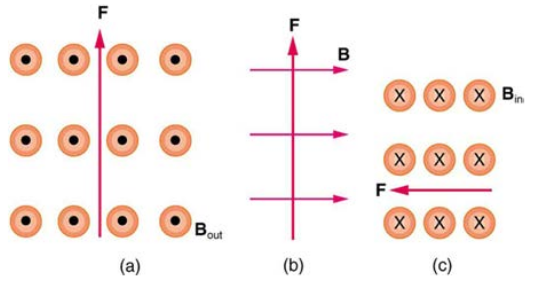
\includegraphics[width=0.75\textwidth]{figures/lorentzProblem.png}
\caption{\label{fig:lorentzProblem} Three different magnetic field and charge scenarios.  The vector $\vec{F}$ is the direction of the Lorentz force, and the magnetic field is uniform.  A dot indicates that the magnetic field is coming out of the page, and an x indicates that the field is going into the page.}
\end{figure}
\end{frame}

\begin{frame}{Magnets and magnetic fields}
\begin{columns}[T]
\begin{column}{0.3\textwidth}
In which of the diagrams is a positively charged particle moving to the left?
\begin{itemize}
\item A: A
\item B: B
\item C: C
\item D: Double WAT
\end{itemize}
\end{column}
\begin{column}{0.7\textwidth}
\begin{figure}
\centering
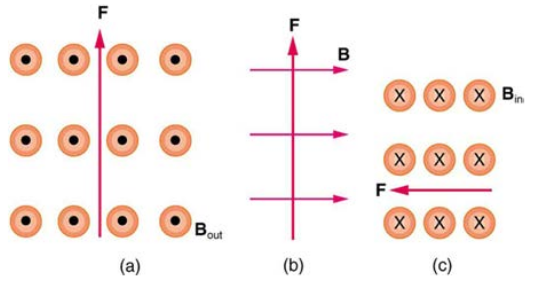
\includegraphics[width=0.75\textwidth]{figures/lorentzProblem.png}
\caption{\label{fig:lorentzProblem2} Three different magnetic field and charge scenarios.}
\end{figure}
\end{column}
\end{columns}
\end{frame}

\begin{frame}{Magnets and magnetic fields}
\begin{columns}[T]
\begin{column}{0.3\textwidth}
In which of the diagrams is a positively charged particle moving upwards?
\begin{itemize}
\item A: A
\item B: B
\item C: C
\item D: Double WAT
\end{itemize}
\end{column}
\begin{column}{0.7\textwidth}
\begin{figure}
\centering
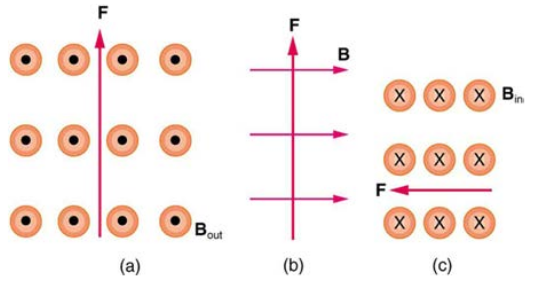
\includegraphics[width=0.75\textwidth]{figures/lorentzProblem.png}
\caption{\label{fig:lorentzProblem3} Three different magnetic field and charge scenarios.}
\end{figure}
\end{column}
\end{columns}
\end{frame}

\begin{frame}{Magnets and magnetic fields}
\begin{columns}[T]
\begin{column}{0.3\textwidth}
In which of the diagrams is a negatively charged particle moving into the page?
\begin{itemize}
\item A: A
\item B: B
\item C: C
\item D: Double WAT
\end{itemize}
\end{column}
\begin{column}{0.7\textwidth}
\begin{figure}
\centering
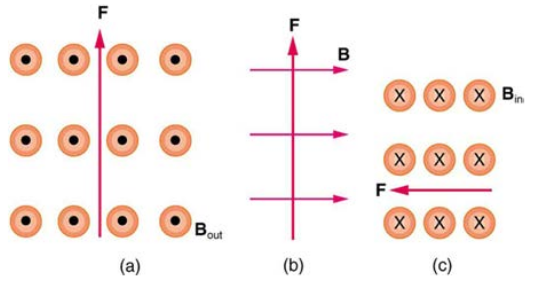
\includegraphics[width=0.75\textwidth]{figures/lorentzProblem.png}
\caption{\label{fig:lorentzProblem4} Three different magnetic field and charge scenarios.}
\end{figure}
\end{column}
\end{columns}
\end{frame}

\begin{frame}{Magnets and magnetic fields}
\begin{columns}[T]
\begin{column}{0.3\textwidth}
In which of the diagrams is a negatively charged particle moving to the right?
\begin{itemize}
\item A: A
\item B: B
\item C: C
\item D: Double WAT
\end{itemize}
\end{column}
\begin{column}{0.7\textwidth}
\begin{figure}
\centering
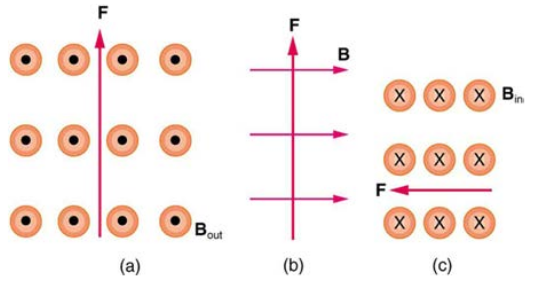
\includegraphics[width=0.75\textwidth]{figures/lorentzProblem.png}
\caption{\label{fig:lorentzProblem5} Three different magnetic field and charge scenarios.}
\end{figure}
\end{column}
\end{columns}
\end{frame}

\begin{frame}{Magnets and magnetic fields}
A theorem for the magnitude of the cross-product:  Let $\vec{a}$ and $\vec{b}$ be vectors and $\theta$ be the angle between them.  The magnitude of the cross-product is
\begin{equation}
|\vec{a} \times \vec{b}| =  a b \sin\theta
\end{equation}
Thus, the magnitude of the Lorentz force is
\begin{equation}
F_{\rm L} = q v B \sin\theta
\end{equation}
The angle $\theta$ is between the velocity and the magnetic field.
\end{frame}

\begin{frame}{Magnets and magnetic fields}
A cosmic ray proton moving toward the Earth at $3 \times 10^{6}$ m/s experiences a magnetic force of $2 \times 10^{-17}$ N. What is the strength of the magnetic field if there is a $45$ degree angle between it and the proton’s velocity?  (Remember that $q$ for a proton is $1.6 \times 10^{-19}$ C).
\begin{itemize}
\item A: 0.1 Gauss
\item B: 0.6 Gauss
\item C: 1 Gauss
\item D: 6 Gauss
\end{itemize}
\end{frame}

\begin{frame}{Magnets and magnetic fields}
\textbf{Other examples:}
\begin{enumerate}
\item Magnetic fields do no work
\item $v = E/B$
\item q/m circle (potential demonstration)
\end{enumerate}
\end{frame}

\begin{frame}{Magnets and magnetic fields}
\begin{figure}
\centering
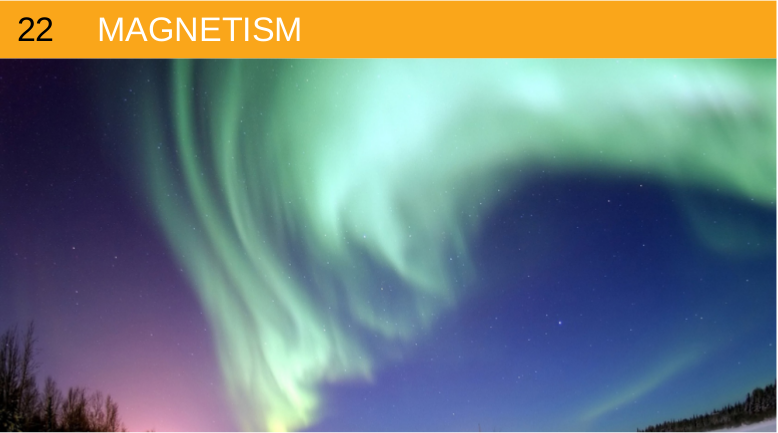
\includegraphics[width=0.9\textwidth]{figures/aurora.png}
\caption{\label{fig:aurora} The aurora borealis, or northern lights.}
\end{figure}
\end{frame}

\begin{frame}{Magnets and magnetic fields}
A cool talk on the aurora borealis:
\url{https://youtu.be/czMh3BnHFHQ} \\
\begin{figure}
\centering
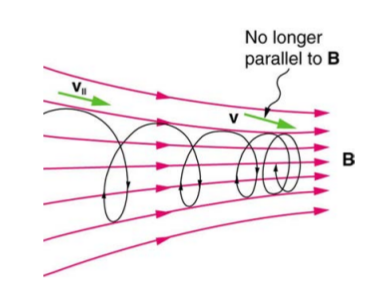
\includegraphics[width=0.45\textwidth]{figures/mag1.png}
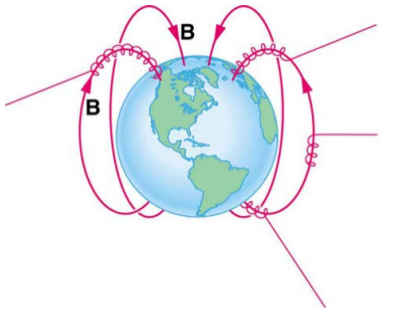
\includegraphics[width=0.45\textwidth]{figures/mag2.png}
\end{figure}
One un-explained piece: what does it mean for the electrons and protons to \textit{high-five} the neutral oxygen and nitrogen atoms?
\end{frame}

\section{Force on a Moving Charges and Current Carrying Conductors}

\begin{frame}{Force on a Moving Charges and Current Carrying Conductors}
Introduction to magnetic forces on current-carrying conductors: \\ \vspace{0.5cm}
\url{https://youtu.be/5fqwJyt4Lus} \\
\begin{figure}
\centering
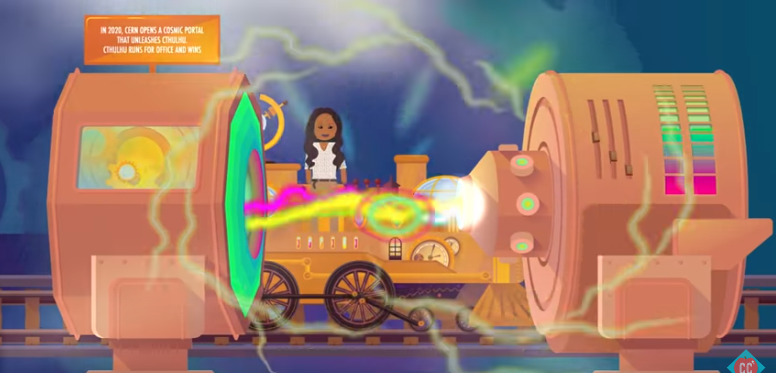
\includegraphics[width=0.7\textwidth]{figures/pbs.png}
\end{figure}
\end{frame}

\begin{frame}{Force on a Moving Charges and Current Carrying Conductors}
\textbf{Charge to mass ratio, and \textit{cyclotrons}.}
\begin{figure}
\centering
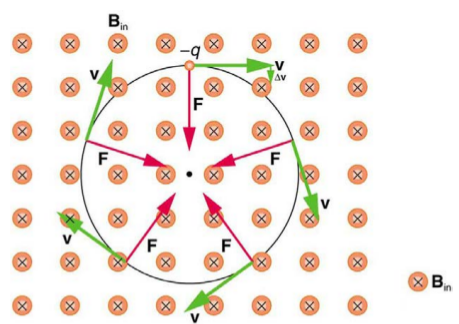
\includegraphics[width=0.6\textwidth]{figures/qmcircle.png}
\caption{\label{fig:qmcircle} The centripetal force is provided by the Lorentz force.}
\end{figure}
\end{frame}

\begin{frame}{Force on a Moving Charges and Current Carrying Conductors}
\textbf{Group exercise}: Suppose we place a gas of unknown particles in the uniform magnetic field of Fig. \ref{fig:qmcircle} and get them moving in a circle.  The angular frequency is 95.5788 MHz, and the B-field is exactly 1.0 T.  (a) Show that the relationship between the angular frequency $\omega$, the B-field strength $B$, and the $q/m$ ratio is $q/m = \omega/B$. (b) With which particle are we dealing?  Is it a proton, a neutron, an electron, or an alpha particle? (\textit{Hint: use the angular frequency and magnetic field to obtain the $q/m$ ratio, and then look up the masses and charges of these particles to make the determination}).
\end{frame}

\begin{frame}{Magnets and magnetic fields}
Two unknown particles are moving in helixes through a region where there is a magnetic field.  Both move clockwise as you observe them. One particle spins around the field line with higher frequency compared to the other.  Which of the following is true?
\begin{itemize}
\item A: The particles are identical; they just had different initial conditions.
\item B: The charge is smaller for the particle with the larger frequency.
\item C: The mass is larger for the particle with the larger frequency.
\item D: The $q/m$ ratio is larger for the particle with the larger frequency.
\end{itemize}
\end{frame}

\begin{frame}{Magnets and magnetic fields}
Which of the following is true of a charged particle moving in a helical fashion through a magnetic field?
\begin{itemize}
\item A: Raising the strength of the B-field increases the period
\item B: Raising the strength of the B-field increases the frequency
\item C: The particle has a constant velocity parallel to the field
\item D: B and C
\end{itemize}
\end{frame}

\begin{frame}{Magnets and magnetic fields}
Two unknown particles are moving in helixes through a region where there is a magnetic field.  One moves clockwise as you observe it, and the other moves counter-clockwise, and the helices have about the same radius.  Which of the following is true?
\begin{itemize}
\item A: The particles have identical charge.
\item B: The particles have identical charge, and the same mass.
\item C: The particles have opposite charge, and the same mass.
\item D: The particles have different masses.
\end{itemize}
\end{frame}

\begin{frame}{Force on a Moving Charges and Current Carrying Conductors}
\textbf{Magnetic containment and \textit{tokamaks}.}
\begin{figure}
\centering
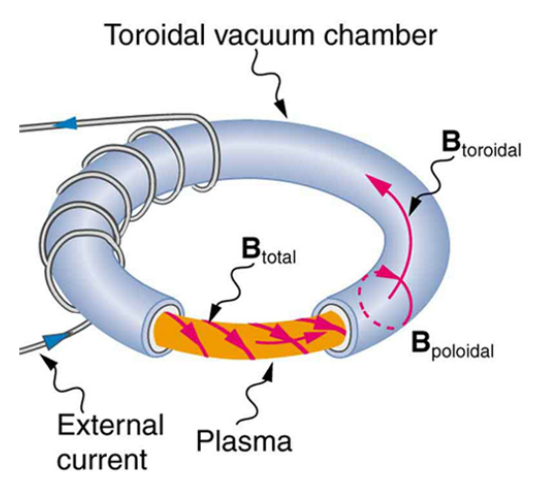
\includegraphics[width=0.5\textwidth]{figures/tokamak.png}
\caption{\label{fig:tokamak} The tokamak contains high-energy plasma, e.g. a charged gas of electrons and protons.}
\end{figure}
\end{frame}

\begin{frame}{Force on a Moving Charges and Current Carrying Conductors}
\textbf{Group exercise}: Suppose $\approx 6.7 \times 10^{12}$ protons are circling through the tokamak at a rate of 0.20 MHz, and the radius of the circle of the tokamak is 20.0 meters.  The radius of the \textit{pipe} of the tokamak is 2.0 m. (a) Work out the \textit{current} $I$ going through the tokamak.  (b) Using $B = \mu_0 I / (2\pi r_{pipe})$, compute the poloidal magnetic field of the current.
\end{frame}

\section{Motors}

\begin{frame}{Motors} 
\begin{figure}
\centering
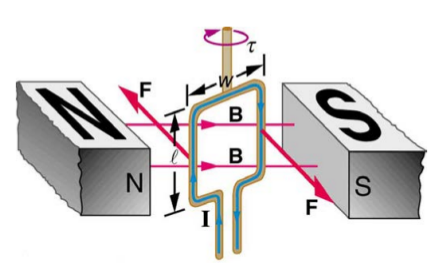
\includegraphics[width=0.6\textwidth]{figures/loop.png}
\caption{\label{fig:loop} In a loop of current in a uniform magnetic field, we find forces going the opposite directions.}
\end{figure}
\end{frame}

\begin{frame}{Motors} 
\begin{figure}
\centering
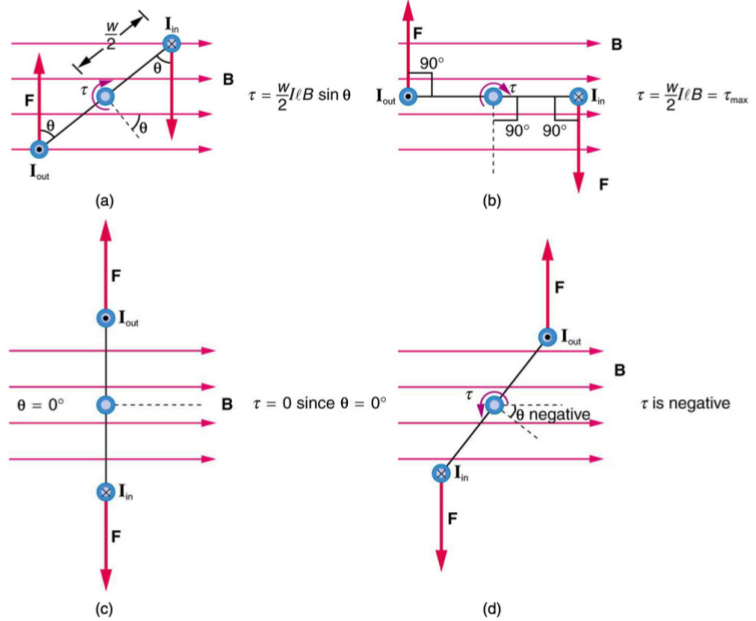
\includegraphics[width=0.6\textwidth]{figures/torque.png}
\caption{\label{fig:loop2} This leads to torque.}
\end{figure}
\end{frame}

\begin{frame}{Motors} 
\begin{figure}
\centering
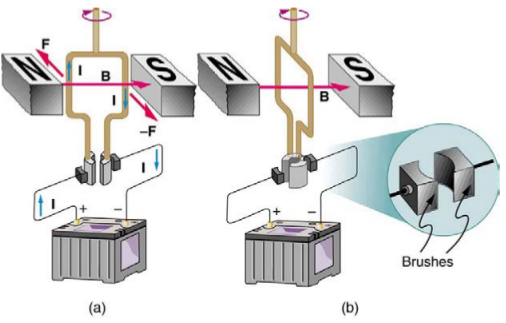
\includegraphics[width=0.6\textwidth]{figures/motor.png}
\caption{\label{fig:loop3} Torque can be used to drive a motor.}
\end{figure}
\end{frame}

\begin{frame}{Motors}
Let the number of loops in the coil be $N$, the current be $I$, the area of the loops be $A$, and the magnetic field be $B$.  The angle between the force and loops is $\theta$.  The magnitude of the torque $\tau$ is
\begin{equation}
\tau = N I A B \sin\theta
\end{equation}
\end{frame}

\begin{frame}{Motors}
At what angle between the loops and the B field is the torque maximized?
\begin{itemize}
\item A: 0 degrees
\item B: 45 degrees
\item C: 90 degrees
\item D: 135 degrees
\end{itemize}
\end{frame}

\begin{frame}{Motors}
Which of the following would boost the torque of a motor?
\begin{itemize}
\item A: Increasing the B-field magnitude
\item B: Decreasing the number of loops
\item C: Increasing the number of loops
\item D: A and C
\end{itemize}
\end{frame}

\begin{frame}{Motors}
Suppose $I = 10$ amps, $B = 0.01$ T, $N = 200$, and the loops have a common radius of 5 cm.  \textbf{Group exercise:} what is the maximum torque?
\end{frame}

\section{The Hall Effect}

\begin{frame}{The Hall Effect}
Negative charge flows in conductors.
\begin{figure}
\centering
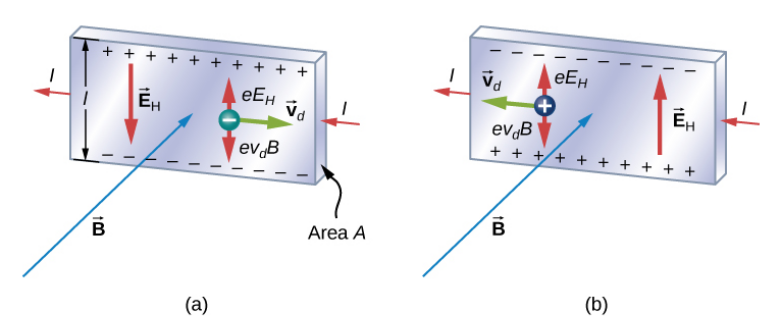
\includegraphics[width=0.7\textwidth]{figures/Hall.png}
\caption{\label{fig:Hall} The Hall effect is an important way to establish that what we call \textit{negative charge} is actually flowing in conductors.}
\end{figure}
\end{frame}

\begin{frame}{The Hall Effect}
Negative charge flows in conductors. \\ \vspace{0.5cm}
``Therefore, by simply measuring the sign of V, we can determine the sign of the majority charge carriers in a metal.
Hall potential measurements show that electrons are the dominant charge carriers in most metals. However, Hall potentials
indicate that for a few metals, such as tungsten, beryllium, and many semiconductors, the majority of charge carriers are
positive. It turns out that conduction by positive charge is caused by the migration of missing electron sites (called holes) on
ions.''
\end{frame}

\begin{frame}{The Hall Effect}
\small
\begin{figure}
\centering
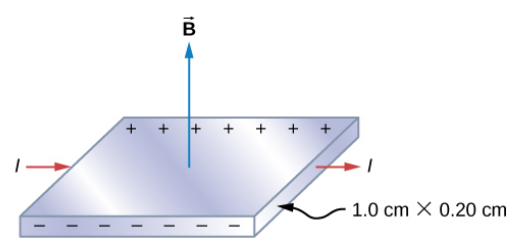
\includegraphics[width=0.6\textwidth]{figures/Hall2.png}
\caption{\label{fig:Hall2} An example of a Hall measurement, with some typical numbers.}
\end{figure}
\begin{itemize}
\item $I = 100$ A
\item $B = 1.5$ T
\item $l = 1.0\times 10^{-2}$ m
\item $n = 5.9 \times 10^{28}$ m$^{-3}$, $e = 1.6 \times 10^{-19}$ C
\item $A = 2.0 \times 10^{-5}$ m$^{2}$
\end{itemize}
\end{frame}

\begin{frame}{The Hall Effect}
\small
\begin{figure}
\centering
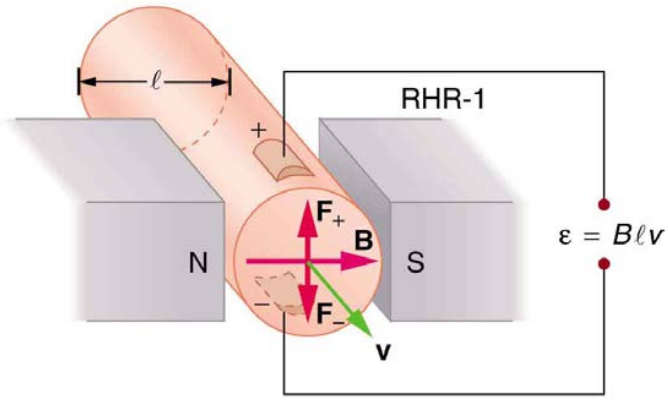
\includegraphics[width=0.45\textwidth]{figures/Hall3.png}
\caption{\label{fig:Hall3} A Hall measurement that is used to measure fluid flow.}
\end{figure}
\textbf{Group exercise:} A Hall effect flow probe is placed on an artery, applying a 0.1 T magnetic field across it, in a setup similar to that in Fig. \ref{fig:Hall3}. What is the blood velocity, given the vessel’s inside diameter is 4.00 mm and the Hall voltage is $0.8 \mu V$?
\end{frame}

\section{Amp\`{e}re's Law}

\begin{frame}{Amp\`{e}re's Law}
\begin{figure}
\centering
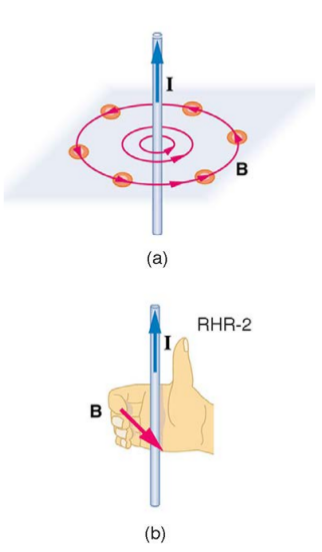
\includegraphics[width=0.3\textwidth]{figures/rhr2.png}
\caption{\label{fig:amp} Magnetic fields creat currents!  To remember the direction, use your right hand.}
\end{figure}
\end{frame}

\begin{frame}{Amp\`{e}re's Law}
Amp\`{e}re's Law states that the current produced by a long straight wire is
\begin{equation}
B = \frac{\mu_0 I}{2\pi r}
\end{equation}
The current is $I$, the distance from the wire is $r$, and $\mu_0 = 4\pi \times 10^{-7}$ T m/A.
\end{frame}

\begin{frame}{Amp\`{e}re's Law}
\textbf{Group exercise:} Suppose we have a wire carrying 1 A, and we are 1 cm away from it.  What is the magnetic field?  What is the magnetic field if another wire is located 1 cm away from us, but carries -1 A? Should the fields add or subtract? \\ \vspace{1cm}
\url{https://youtu.be/1JZLKvWO0ks}
\end{frame}

\begin{frame}{Amp\`{e}re's Law}
\begin{figure}
\centering
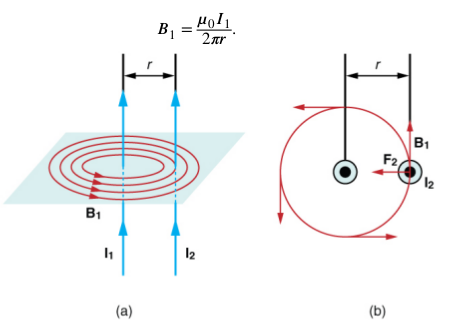
\includegraphics[width=0.5\textwidth]{figures/amp.png}
\caption{\label{fig:amp2} Definition of the amp is derived from this setup.}
\end{figure}
\end{frame}

\begin{frame}{Amp\`{e}re's Law}
The B-field at wire 2 due to wire 1 is
\begin{equation}
B_1 = \frac{\mu_0 I_1}{2\pi r}
\label{eq:B}
\end{equation}
The force on wire 2 is 
\begin{equation}
F_2 = I_2 l B_1
\end{equation}
Dividing both sides by $l$ and substituting in Eq. \ref{eq:B}, we have
\begin{equation}
\frac{F}{l} = \frac{\mu_0 I_1 I_2}{2\pi r}
\end{equation}
\textbf{Group board exercise:} let $I_1 = I_2 = 1.0$ A, and $r = 1$ meter.  What is the force per unit length $F/l$?  (Recall that $\mu_0 = 4\pi \times 10^{-7}$ T m/A by definition).
\end{frame}

\section{Magnetic Fields and Work}

\begin{frame}{Magnetic Fields and Work}
Notice from the Lorentz force that magnetic fields do not perform work:
\begin{align}
\vec{F} &= q \vec{v} \times \vec{B} \\ 
\vec{v} t &= \vec{x} \\
\vec{F} &= \frac{q}{t} \vec{x} \times \vec{B} \\
W &= \vec{x} \cdot \vec{F} \\
W &= \frac{q}{t} \vec{x} \cdot \left( \vec{x} \times \vec{B} \right)
\end{align}
\end{frame}

\begin{frame}{Magnetic Fields and Work}
In the final step, why is the right hand side $\left(\vec{x} \cdot \left( \vec{x} \times \vec{B} \right) \right)$ zero?
\begin{itemize}
\item A: Because $\vec{x}$ is parallel to $\vec{x} \times \vec{B}$.
\item B: Because $\vec{x}$ is perpendicular to $\vec{x} \times \vec{B}$.
\item C: Because $q = 0$ on average.
\item D: Because $\vec{x}$ is perpendicular to $\vec{B}$.
\end{itemize}
\end{frame}

\section{PHeT: Electromagnets}

\begin{frame}{PHeT: Electromagnets}
\begin{figure}
\centering
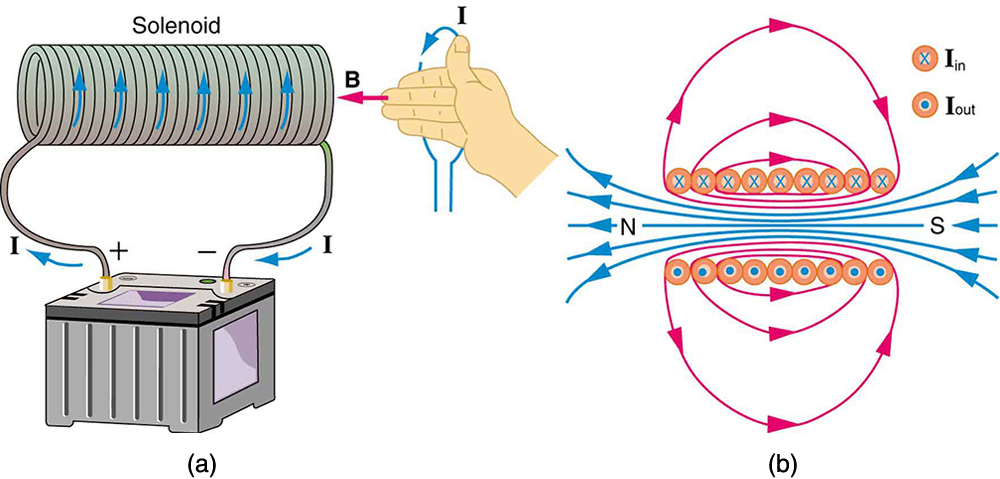
\includegraphics[width=0.75\textwidth]{figures/solenoid.jpeg}
\caption{\label{fig:solenoid1} A solenoid is an application of Amp\`{e}re's Law.}
\end{figure}
\end{frame}

\begin{frame}{PheT: Electromagnets}
Follow the link: \\ \vspace{0.5cm}
\url{https://phet.colorado.edu/en/simulation/magnets-and-electromagnets}
\end{frame}

\begin{frame}{PHeT: Electromagnets}
\small
\begin{enumerate}
\item Click on the electromagnet tab, and hide the field and compass using the menu in the upper right.  Also, display the magnetometer.
\item Place the magnetometer to one side of the \textit{solenoid.}  Work out the relationship between the magnetic field strength and voltage.  Is it linear, quadratic, or something else?
\item Assuming the circuit has some fixed resistance, is the relationship between current and field strength linear?  Why or why not?
\item Now fix the voltage and vary the number of loops.  Work out the relationship between magnetic field strength and loop number.  Is it linear, quadratic, or something else?
\item Propose an equation for $B_{solenoid}$ based on the prior measurements.
\end{enumerate}
\end{frame}

\begin{frame}{Force on a Moving Charges and Current Carrying Conductors}
\textbf{Electromagnets.}
\begin{figure}
\centering
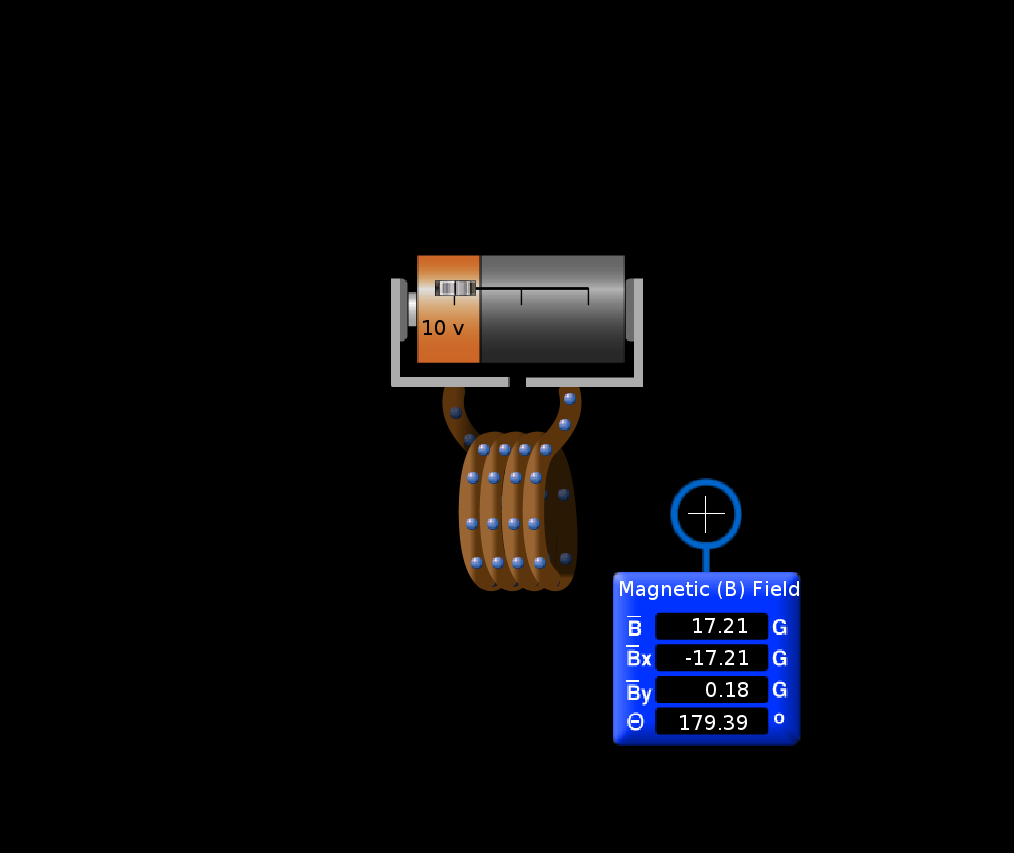
\includegraphics[width=0.5\textwidth]{figures/phetemmag.png}
\caption{\label{fig:phetemmag} The electromagnet converts charge to magnetic field strength.}
\end{figure}
\end{frame}

\begin{frame}{Force on a Moving Charges and Current Carrying Conductors}
The result should be something like:
\begin{align}
B &\propto N I \\
B &= \mu_0 n I
\end{align}
\begin{itemize}
\item $n$: Number of turns per unit length (because we can always change the density and get a different answer).
\item $I$: Current
\item $\mu_0$: Magnetic permeability of free space (solenoid is empty).
\item \textbf{Now switch to AC current on the voltage supply.  What happens to the field?}
\item \textbf{What would happen in another unconnected solenoid placed \textit{next} to the oscillating solenoid?}
\end{itemize}
\end{frame}

\section{Conclusion}

\begin{frame}{Unit 2 Summary}
\textbf{Reading: Chapter 22}
\begin{enumerate}
\item Magnets and magnetic fields
\item Force on a moving charge in a magnetic field
\item \textbf{The Hall effect}
\item Magnetic forces on conductors
\item \alert{Amp\`{e}re's Law}
\end{enumerate}
\end{frame}

\end{document}
